\section{Scalability Plugin}

MANO framework faces scalability challenges in large-scale deployments. The amount of infrastructure a single instance of MANO framework can manage is limited. The scaling of MANO should be addressed to avoid it from being the bottleneck in the NFV paradigm. \\

We propose a hierarchical scaling mechanism for MANO by implementing and evaluating a scalability plugin (SPL) in pishahang. SPL adds the following features to pishahang 1) Spawn/Terminate child MANO instances, 2) State management between instances, 3) Redirection of requests from parent instance to child instances and 4) Monitoring of system load on all instances

\subsection{Architecture}

SPL is built based on the "base plugin framework" of SONATA. The figure \ref{fig:pmdesign} from SONATA documentation shows the high-level architecture of the SONATA MANO framework. The plugins communicate over the message broker using AMQP with other plugins and together facilitate the functions of MANO.

\begin{figure}[h]
	\centering
	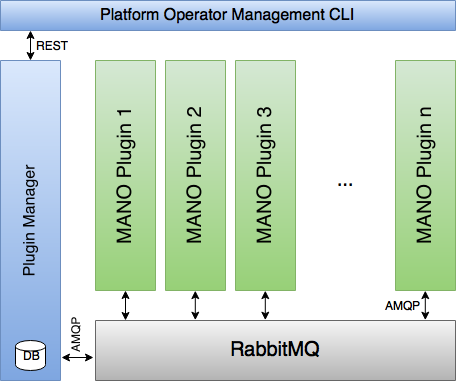
\includegraphics[width=0.7\linewidth]{figures/pm_design}
	\caption{SONATA MANO plugin architecture}
	\label{fig:pmdesign}
\end{figure}

The architecture of the scalability plugin is shown in the figure \ref{fig:scalingarch}. SPL mainly consists of 1) \textbf{Scaling Manager:} is responsible for the overall workflow of the SPL, which includes monitoring, spawning, termination and state management of MANO instances. 2) \textbf{MANO Manager:} is responsible for sending the on-boarding and instantiation requests to the parent MANO using python-mano-wrappers. SPL co-ordinates with the service lifecycle management plugin in pishahang to provide the features discussed above. The workflow of this is discussed in the further sections. 

\subsubsection{Scaling Manager}

Features of the scaling manager are discussed briefly in this section. 

\subsubsection*{Monitoring}

SPL needs to continuously monitor the system resource utilization and take scaling decisions based on that. We are using the \textit{average system load} values given by the linux kernel for taking the scaling decisions. System load is the number of processes which are being executed by the CPU or in waiting state. The linux kernel provides 3 average values of system load calculated over a period of 1, 5 and 15 minutes. \\

As a proof of concept, SPL uses \textit{5m} and \textit{15m} moving averages as a heuristic for scaling decisions. \textit{1m} average is not considered to avoid taking decisions on a short lived spike in system load. SPL has the following simple rule set listed below, note that the configurable threshold value is used to take relevant actions. For simplicity, we consider "0.7" as the threshold value as it is generally used in the wild by system administrators. 

\begin{enumeratelist}

\begin{itemize}
	\item{\textbf{Rule 1}\\} If \textit{5m} load average is more than the \textit{threshold} value, then, SPL will consider this as a warning sign and start preparing a child MANO instance.
	\item{\textbf{Rule 2}\\} If \textit{15m} load average is more than the \textit{threshold} value, then, SPL will consider this as a critical sign and start redirecting service requests on the parent mano to the child MANO instance.
	\item{\textbf{Rule 3}\\} If \textit{15m} load average of both the parent and child instances are less than the \textit{threshold} value, then, SPL will consider this as decreasing load and terminate the child MANO instance.

\end{itemize}
\caption{Scaling Plugin Rules}
\label{list:splrules}
\end{enumeratelist}


\subsubsection*{SLM Communication}

The monitoring of the load information happens in the SPL, however, the service requests are handled by the SLM plugin. SLP communicates information about the current load of the instances to the SLM and based on this response, SLM decides whether to continue serving the request or to forward it to one of the child MANOs.

The forwarding logic is implemented on the SLM plugin of pishahang. The forwarding logic includes on-boarding the VNFD/NSD and instantiating it.

\subsubsection*{Spawning}

Spawning refers to the action of instantiating a child instance of pishahang by allocating new physical resources on existing infrastructure. According to Rule 1 from \ref{list:splrules}, when the threshold is reached, a request to instantiate a new instance is sent to the Mano Manager. Mano Manager will instantiate a new instance of pishahang and returns the IP address of the newly deployed instance. This new instance is now added to the list of child MANO instances and continuously monitored.
 

\subsubsection*{Termination}

Once the load on the parent MANO and child MANO instances are reducing, it becomes unnecessary and expensive to use the allocated physical resources of the child MANO. According to Rule 3 from \ref{list:splrules}, the termination request of the child MANO is sent to the MANO Manager and the metadata generated by the child instances are saved on the parent instance. Metadata that is saved includes the VNF records and network service records.


\subsubsection{MANO Manager}
MANO Manager is responsible for the end communication with the parent MANO. MANO Manager receives an instantiation request from the Scaling Manager and uses python-mano-wrappers to make an instantiation request to the parent MANO to instantiate a child MANO instance. 

MANO Manager will wait for successful instantiation of the instance and return the IP address of the instance to the Scaling Manager.

\subsubsection*{Service Descriptors}

We designed a basic function descriptor and service descriptor in the schema supported by the pishahang MANO framework. The descriptors are stored as part of the scaling plugin and used by the MANO Manager to on-board and instantiate upon request. We have created the descriptors for both OSM and Pishahang.

\subsubsection*{MANO Image}

A Virtual Machine (VM) image with MANO pre-installed is used along with the service descriptors to spawn new instances of MANO. As a proof of concept, we have created images with OSM and pishahang. However, the pishahang image that was created was unstable and has unexpected behavior. These images are first created locally and later uploaded to the VIM where the instances will be created. In our tests we used OpenStack as our VIM.

\begin{figure}[h]
	\centering
	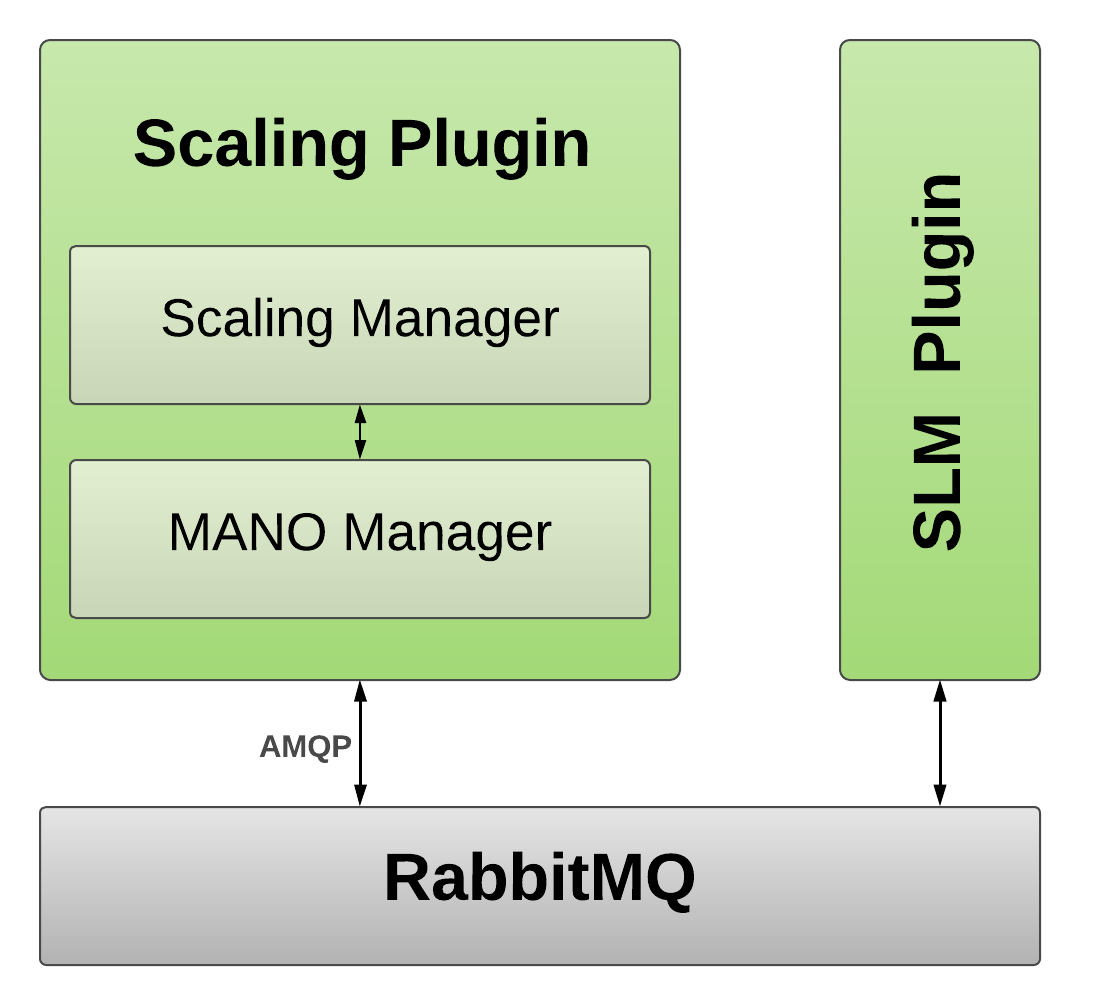
\includegraphics[width=0.7\linewidth]{figures/scalingarch}
	\caption{Scaling plugin architecture}
	\label{fig:scalingarch}
\end{figure}


\subsection{Workflow}

\begin{figure}[h]
	\centering
	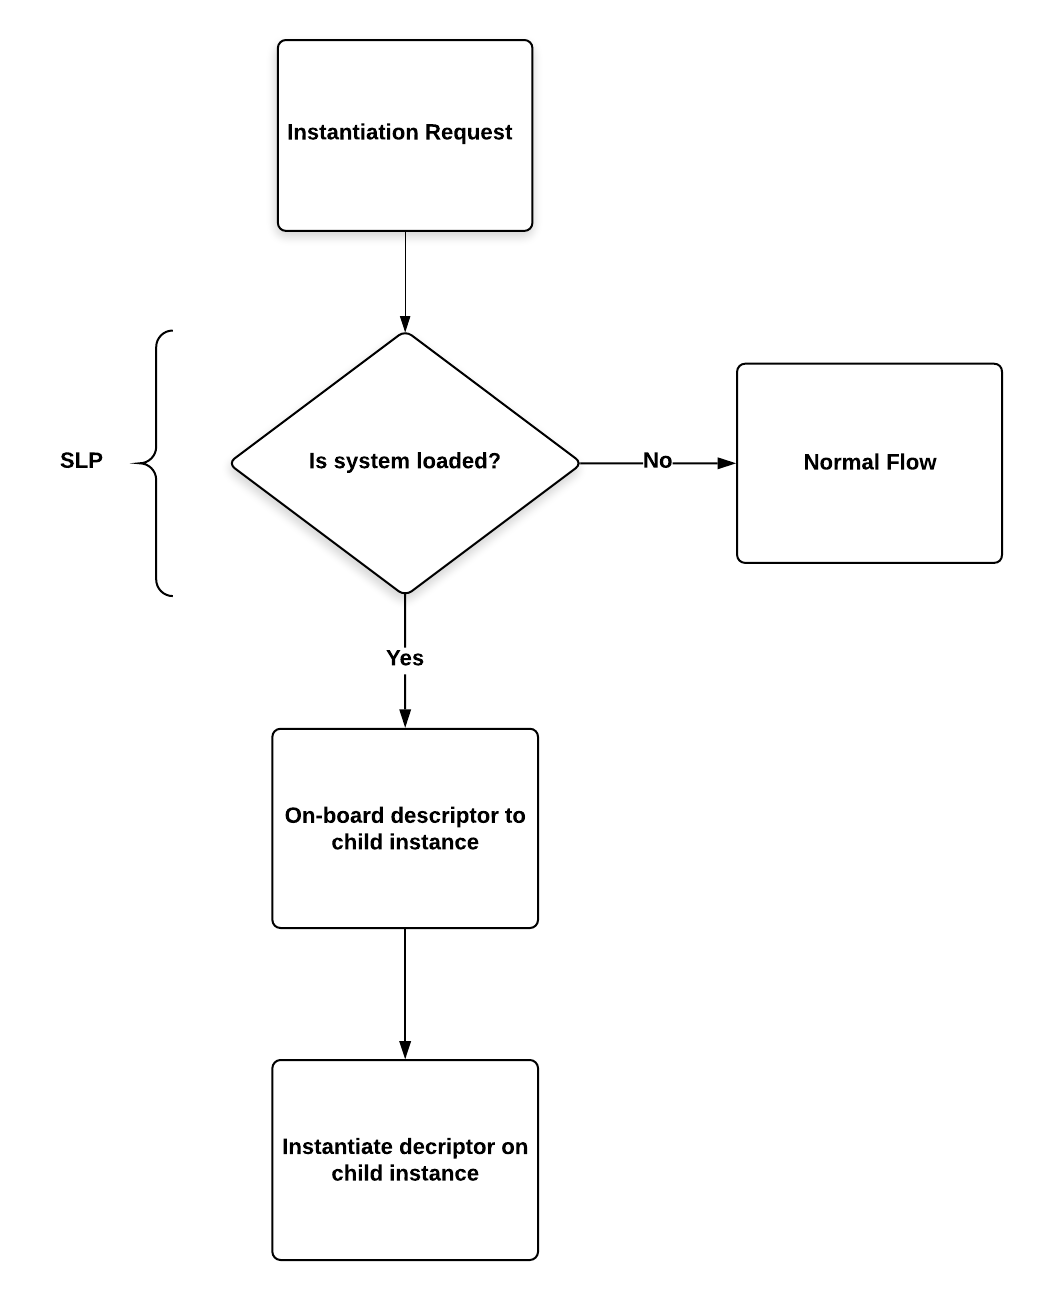
\includegraphics[width=0.8\linewidth]{figures/SLPSLMWorkflow}
	\caption{Service Lifecycle Manager with Scaling Plugin Workflow}
	\label{fig:slpslmworkflow}
\end{figure}


\begin{figure}[h]
	\centering
	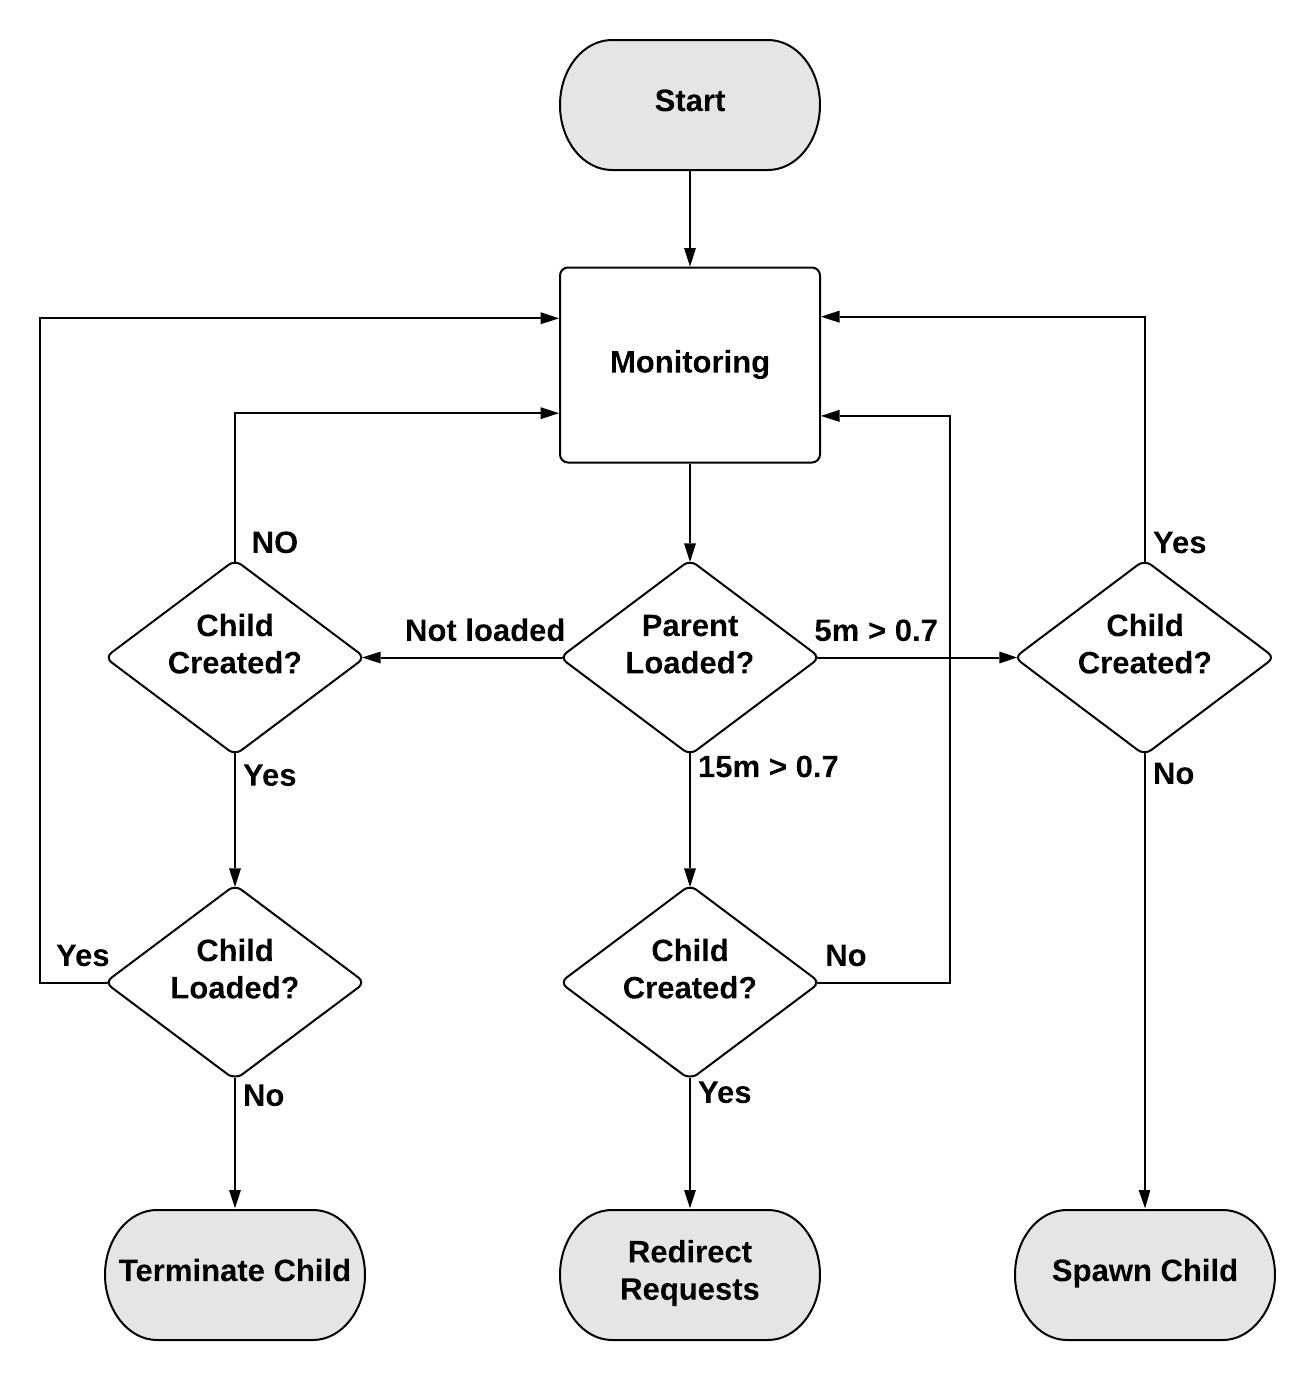
\includegraphics[width=1\linewidth]{figures/SPLWorkflow}
	\caption{Scaling Plugin Workflow}
	\label{fig:splworkflow}
\end{figure}

